\documentclass[fleqn,11pt]{article}

\usepackage[left=2cm,right=2cm,
top=1.25cm,
bottom=0.5cm,%
headheight=11pt,%
letterpaper]{geometry}



\usepackage[left=2cm,right=2cm,
			top=1.25cm,
			bottom=2.25cm,%
			headheight=11pt,%
			letterpaper]{geometry}
			

\frenchspacing			

\nonstopmode



\usepackage{lmodern}
\usepackage[T1]{fontenc}
\usepackage[utf8]{inputenc}

%\usepackage[sfdefault]{roboto}
\usepackage[sfdefault,light]{roboto}


\usepackage{noweb}

\usepackage{multicol}
\usepackage{fancyhdr}
\usepackage{blindtext,graphicx}
\usepackage[absolute]{textpos}
%\usepackage[parfill]{parskip}
\usepackage{parskip}
\setlength{\parskip}{\baselineskip}

\usepackage[colorlinks=true,urlcolor=blue,citecolor=brown, urlbordercolor=black]{hyperref}


\makeatletter
\Hy@AtBeginDocument{%
	\def\@pdfborder{0 0 1}% Overrides border definition set with colorlinks=true
	\def\@pdfborderstyle{/S/U/W 0.5}% Overrides border style set with colorlinks=true
	% Hyperlink border style will be underline of width 1pt
}
\makeatother

\usepackage{gensymb}
\usepackage{csquotes}
\usepackage{amsmath}
\usepackage{fontawesome}
\usepackage{orcidlink}
\usepackage{standalone}
\usepackage{pdfpages}
\usepackage{subfiles}
\usepackage{svg}
\listfiles
\svgpath{{../biology/simulation/GROMACS/BUMPy_bilayer/data/}{../electronics/propagation/}}

\usepackage{sidecap}
\usepackage{float}
\usepackage{amssymb}
\usepackage{textcomp}
\usepackage{lettrine}

\usepackage{subfig}


\setlength{\footnotesep}{0.7\baselineskip}



% This allows the endnote and reference footnotes to float with the text.
%\usepackage{enotez}
%\let\footnote\endnote
%\let\footnotetext\endnotetext
%\let\footnotemark\endnotemark

\usepackage{soul} % strikethrough \st


%\usepackage{draftwatermark}
%\SetWatermarkText{DRAFT}
%\SetWatermarkScale{0.25}

\usepackage{booktabs,caption}
\usepackage[flushleft]{threeparttable}

%\usepackage{biblatex}
\usepackage[backend=bibtex8, sorting=none, style=phys]{biblatex}
% style=chem-angew
\let\cite\footfullcite



%\let\cite\footcite

\addbibresource{references.bib}
%biblatex has a zoterordfxml
% might avoid the need for python bibtex_collections.py



\usepackage{etoolbox}
\AtBeginEnvironment{quote}{\small}




\usepackage{pifont}
\newcommand{\cmark}{\ding{51}}%
\newcommand{\xmark}{\ding{55}}%


\newcommand{\wikinote}[1]{\textsuperscript{[\color{blue}{\textit{\textbf{#1}}}]}}
\newcommand{\citationneeded}[1][]{\textsuperscript{[\color{blue}{\it \bf{citation needed}#1}]}}
\newcommand{\dubiousdiscuss}[1][]{\textsuperscript{\color{blue} [{\it \bf{dubious-discuss}}]} }

\newcommand{\light}[1]{\textcolor{gray}{#1}}

\newcommand{\ntilde}{\char`~}

%
%
\usepackage{titlesec}
%
%% custom section


\titleformat{\section}
{\normalfont\LARGE\bfseries}{\thesection}{1em}{}
%\titleformat{\section}
%{\normalfont\LARGE\bfseries\PRLsep}
%{{{{\itshape \thesection\hskip 9pt\textpipe\hskip 9pt}}}}{0pt}{}

%% custom section
%\titleformat{\subsection}
%{\normalfont\Large\bfseries\PRLsep}
%{{{{\itshape \thesection\hskip 9pt\textpipe\hskip 9pt}}}}{0pt}{}
%
%
%


\newcommand{\Wsqm}{$\text{ W/m}^2$}

\newcommand{\ghfile}[1]{\href{https://github.com/0xDBFB7/covidinator/tree/master/#1}{\faGithub/\url{#1} }}

%\newcommand{\supercite}[1]{}
%\newcommand{\supercollect}[1]{}


\newlength{\PRLlen}
\newcommand*\PRLsep[1]{{\itshape \Large\settowidth{\PRLlen}{#1}\advance\PRLlen by -\textwidth\divide\PRLlen by -2\noindent\makebox[\the\PRLlen]{\resizebox{\the\PRLlen}{1pt}{$\blacktriangleleft$}}\raisebox{-.5ex}{#1}\makebox[\the\PRLlen]{\resizebox{\the\PRLlen}{1pt}{$\blacktriangleright$}}\bigskip}}


\renewcommand{\thefootnote}{\textcolor{blue}{[\arabic{footnote}]}}

\usepackage{multirow}



\usepackage{graphicx}
\graphicspath{ {../media/} 
				{../firmware/eppenwolf/runs/sic_susceptor/} 
				{../biology/simulation/GROMACS/BUMPy_bilayer/data/}
			}


\usepackage{tcolorbox}
\newtcolorbox{protocol}{colback=yellow!5!white,colframe=yellow!75!black}
\newtcolorbox{equipment}{colback=orange!5!white,colframe=orange!75!black}
\newtcolorbox{autem}{colback=red!5!white,colframe=red!75!black}
\newtcolorbox{toolchain}{colback=blue!5!white,colframe=blue!40!black!40}
\newtcolorbox{sidenote}{colback=cyan!5!white,colframe=blue!40!black!40}
%https://tex.stackexchange.com/questions/66154/how-to-construct-a-coloured-box-with-rounded-corners

%\usepackage[sfdefault,light]{roboto}

\setlength{\TPHorizModule}{1cm}
\setlength{\TPVertModule}{1cm}





%%%%********************************************************************
% fancy quotes
\definecolor{quotemark}{gray}{0.7}
\makeatletter
\def\fquote{%
	\@ifnextchar[{\fquote@i}{\fquote@i[]}%]
}%
\def\fquote@i[#1]{%
	\def\tempa{#1}%
	\@ifnextchar[{\fquote@ii}{\fquote@ii[]}%]
}%
\def\fquote@ii[#1]{%
	\def\tempb{#1}%
	\@ifnextchar[{\fquote@iii}{\fquote@iii[]}%]
}%
\def\fquote@iii[#1]{%
	\def\tempc{#1}%
	\vspace{1em}%
	\noindent%
	\begin{list}{}{%
			\setlength{\leftmargin}{0.05\textwidth}%
			\setlength{\rightmargin}{0.05\textwidth}%
		}%
		\item[]%
		\begin{picture}(0,0)%
		\put(-15,-5){\makebox(0,0){\scalebox{3}{\textcolor{quotemark}{``}}}}%
		\end{picture}%
		\begingroup\itshape}%
	%%%%********************************************************************
	\def\endfquote{%
		\endgroup\par%
		\makebox[0pt][l]{%
			\hspace{0.8\textwidth}%
			\begin{picture}(0,0)(0,0)%
			\put(15,15){\makebox(0,0){%
					\scalebox{3}{\color{quotemark}''}}}%
			\end{picture}}%
		\ifx\tempa\empty%
		\else%
		\ifx\tempc\empty%
		\hfill\rule{100pt}{0.5pt}\\\mbox{}\hfill\tempa,\ \emph{\tempb}%
		\else%
		\hfill\rule{100pt}{0.5pt}\\\mbox{}\hfill\tempa,\ \emph{\tempb},\ \tempc%
		\fi\fi\par%
		\vspace{0.5em}%
	\end{list}%
}%
\makeatother



\titlespacing{\section}{0pt}{\parskip}{0\parskip}
\titlespacing{\subsection}{0pt}{\parskip}{0\parskip}
\titlespacing{\subsubsection}{0pt}{\parskip}{0\parskip}






%%%%********************************************************************
%title link to doi
\newbibmacro{string+doiurlisbn}[1]{%
	\iffieldundef{doi}{%
		\iffieldundef{url}{%
			\iffieldundef{isbn}{%
				\iffieldundef{issn}{%
					#1%
				}{%
					\href{http://books.google.com/books?vid=ISSN\thefield{issn}}{#1}%
				}%
			}{%
				\href{http://books.google.com/books?vid=ISBN\thefield{isbn}}{#1}%
			}%
		}{%
			\href{\thefield{url}}{#1}%
		}%
	}{%
		\href{https://doi.org/\thefield{doi}}{#1}%
	}%
}

\DeclareFieldFormat{journaltitle}{\usebibmacro{string+doiurlisbn}{\mkbibemph{#1}}}



\usepackage{xhfill}


\newcommand{\ressection}[1]{\textbf{{\Large \textit{#1}}}\xrfill[0.1ex]{0.6pt}}

\newcommand{\sk}[1]{\textcolor{orange}{#1}}
\newcommand{\tec}[1]{\textcolor{olive}{\textbf{#1}}}

\newcommand{\itemoptions}{\setlength{\itemindent}{-10pt} \setlength\itemsep{-1em}}

\captionsetup[subfigure]{labelformat=empty}

\begin{document}



%
%
%Daniel Correia\\
%20 Silver Glen Blvd,\\
%Collingwood, Ontario, Canada\\
%L9Y 0G9\\
%
%
%
%\vspace{3 cm}
%\noindent\par
%\noindent\makebox[\textwidth][c]{%
%\begin{minipage}{0.8\textwidth}
%
%\end{minipage}}
%
%
%
%
%\restoregeometry
%
%
%\clearpage

% remember to rename file by name!

\begingroup
\fontseries{t}\selectfont

{\Huge Hi, I'm Daniel!}

\endgroup

\light{\large \textit{Science rules!}}

%{
%\centering
\begin{center}
\small{{Daniel Correia}\ \orcidlink{0000-0002-9353-0216} 
	\let\orighref\href%don't put a link icon next to the orcid
	\renewcommand{\href}[2]{\orighref{#1}{#2\,{\footnotesize{\faExternalLink}}}}
	| \href{https://github.com/0xDBFB7}{github.com/0xDBFB7} | therobotist@gmail.com \textit{(preferred)} | @0xDBFB7 | 1-705-606-8866}\\
%\light{\makebox[\linewidth]{\rule{\textwidth}{0.4pt}}} - add if education moved back up
\end{center}
% dcorreia@whimsysciences.com

\let\orighref\href%don't put a link icon next to the orcid
\renewcommand{\href}[2]{\orighref{#1}{#2\,{\footnotesize{\faExternalLink}}}}


\ressection{SafeSump Inc.}

Co-founder and CTO of a project to design and manufacture a failure-resistant internet-connected water pump system to reduce the incidence of flooding in homes.\\\\ Together with a partner company specializing in hydrogeology, we simultaneously collected and analyzed data from the systems in an attempt to better inform municipalities on groundwater flow.%Granted US Patents \href{https://patents.google.com/patent/US10634146B2/en}{10,634,146} and \href{https://patents.google.com/patent/US11073154B2/en}{11,073,154}. Tremendous dislike of patents and IP protection.

Obtained \$37,500 \textit{Ontario Centres of Excellence} \href{https://drive.google.com/file/d/1WXrxVwTggaL7WEvLv6DgJ891fSo7LqqP/view?usp=sharing}{grant \#26828} (2016-2020) and fulfilled \$75,000 \textit{Federation of Canadian Municipalities} \href{https://drive.google.com/file/d/11pdJNzYDE-28X3m0rH8mE4cxoliTJZGH/view?usp=sharing}{contract} (2018-2020) to develop and install systems in 50 homes.

I was responsible for:
\begin{itemize}\itemoptions
\item Developing backend data collection API (\sk{Python}, \sk{Linux}+\sk{Apache} stack, \sk{PostgreSQL}, \sk{Git}) %web UI design
\item Hardware design and SMD prototyping for embedded electronic controller (\sk{KiCAD} and \sk{Eagle})
\item Pair programming secure firmware and OTA system (\sk{embedded C} and \sk{C++} on STM32 and SAM4, \sk{make}, \sk{bash})
\item Frontend work on a user-facing dashboard to view pump status and modify settings (\sk{HTML}, \sk{JS})
\item Conducting presentations and reporting to partners
\item Developing data analysis, replication, filtering algorithms (\sk{Python}, \sk{gnuplot})
\item Managing production processes, asset tracking, hardware-in-the-loop test systems
\item Creating test cells and batch programming systems for custom capacitive and \href{https://github.com/0xDBFB7/UltimateUltrasonicAmplifier}{ultrasonic} sensors
\end{itemize}
%\setlength{\columnseprule}{0.4pt}
%\columnbreak


\begin{figure}[H]
	%	\makebox[\textwidth][c]{
	\centering
	\captionsetup{labelformat=empty}
	
	\subfloat[][]{
		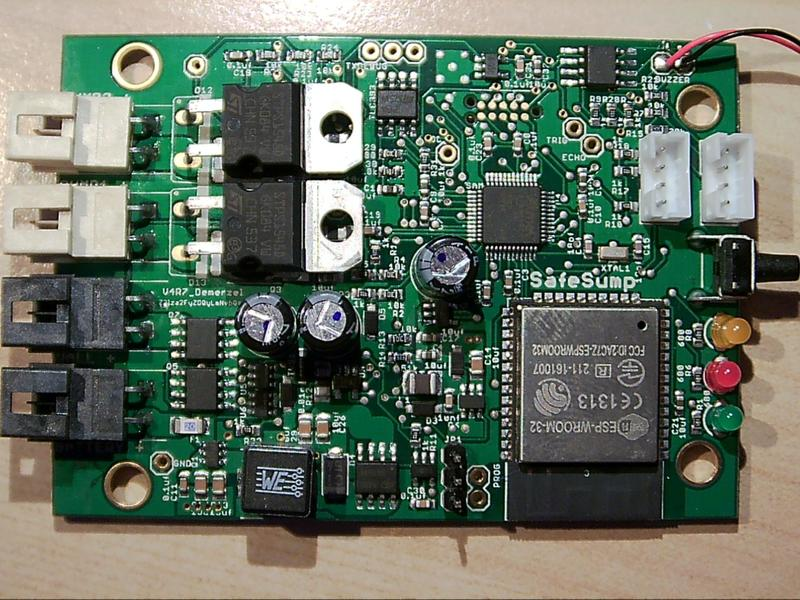
\includegraphics[height=0.2\textwidth]{image1}
	}
	\subfloat[]{
		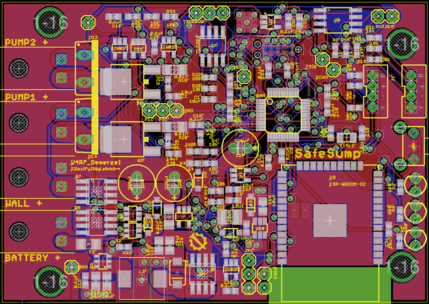
\includegraphics[height=0.2\textwidth]{safesump.png}
	}
	\caption*{Controller designed for SafeSump Inc.}
	\hfill
\end{figure}

%\light{\makebox[\linewidth]{\rule{\textwidth}{0.4pt}}}

\begin{tcolorbox}
	\textbf{Education:} B.Sc. in Science from York University. Graduated January 2021. \href{https://learner.mycreds.ca/#/sharelink/b664abe7-53a7-4d64-a0f1-bef16337edd0/57724eeb-34ab-4b79-b2a6-cd6bc311039e}{\textit{[verify diploma]}} \\
	{\small(Emphasis on electrical engineering, computer science, experimental physics, statistics, chemistry, mathematics, misc)}
\end{tcolorbox}
% add more grade details
 
\pagebreak

\ressection{Projects and skills}

I believe I have experience contributing to broad, highly interdisciplinary projects with limited guidance.

For example, one recent project involved:
%I believe I have experience independently learning and applying skills as needed to effectively contribute to broad, highly interdisciplinary projects. 
%Fully independently designed and carried out an 18-month experiment in the field of bioelectrics on a tight budget, involving
\begin{itemize}\itemoptions
	\item A \href{https://github.com/0xDBFB7/fluorescence_photon_counting/releases/download/v0.01/fluorescence.pdf}{custom synchronous photon counting fluorescence system}, capable of detecting less than a nanogram of dsDNA without amplification (\sk{MAX10 and Cyclone IV FPGAs}, \sk{Verilog HDL})
	\item Custom FDTD electromagnetic simulation software, \href{https://github.com/flaport/fdtd/pull/27}{now contributed upstream} (\sk{PyTorch})
	\item Scientific programming with JuliaLang, analysis with Python, symbolic mathematics with Maxima, SymPy, Mathematica, MATLAB
	\item Developing a custom 12 GHz microwave spectrometer and automated microfluidic sampling system
	\item Technical writing, documentation in \sk{LaTeX}, \sk{Jupyter notebooks}, bibliography management with Zotero and Refbase
%	\item Data visualization with Paraview, Chimera analysis with \sk{Python}
	%	\item Reviewing some 5,000 pages of scientific literature spanning 2,300 papers, highlighting 157 cited
	\item CAD/CAM mechanical design and CNC mill and lathe operation
	\item Molecular dynamics simulation with GROMACS
	%	\item BSL-1 microbiology with E. coli B and T4 bacteriophage culture and plaque assays
	\item Managing import paperwork, safety, and disposal of chemical reagents
	\item Negotiating material transfer agreements for datasets
	\item Collaborating and consulting with subject-matter experts
\end{itemize}



%\pagebreak

Other representative projects include:

%\href{https://github.com/0xDBFB7/ionprinter/}{0xDBFB7/ionprinter/}: A cursory exploration of high-current ion beam lithography techniques. 

%Led to the following spinoff projects:
\begin{itemize}\itemoptions
	\item \href{https://github.com/0xDBFB7/Nyion}{Nyion}: a custom GPU-accelerated plasma simulation program using the particle-in-cell method on a custom block-structured mesh data structure for high computational efficiency\\
	(\sk{C++}, \sk{cmake}, \sk{OpenGL}, \sk{gTest}, minor \sk{HPC} with \sk{CUDA}, \sk{OpenCL}, \sk{OpenMP}+4.5 offload)
	\item An inexpensive \href{https://0xdbfb7.com/furnace.html}{furnace} capable of sintering oxide ceramics: an attempt to make various high-performance ceramic techniques available to a broader audience%, built on the work of more than 200 scientific papers. 
	\item An \href{https://github.com/0xDBFB7/varian-turbo-controller}{inexpensive aftermarket controller} for the Varian Turbo-V series of turbomolecular pumps 
	\item \href{https://gist.github.com/0xDBFB7/7bd7048c6639270e6f291a2673903184}{Control software} for an Inficon BPG-400 vacuum gauge
\end{itemize}





%Preliminary technical report available at doi:\href{https://doi.org/10.5281/zenodo.4568506}{10.5281/zenodo.4568506}



\ressection{Kesti Engineering Ltd.}

Occasional board-level repair of Mazak and Haas CNC machines. A successful repair is documented \href{https://0xdbfb7.com/meldas.html}{here}.

\ressection{Notable deficiencies of experience}

I have completed real-world projects using each of the listed technologies and others not listed, and I am confident that I can contribute to any of the subjects listed above. However, there are also certain large fields which would require some time expenditure to work efficiently.\\ Some examples of fields for which more experienced candidates likely exist include advanced physics or mathematics, organic chemistry, the R language, or FORTRAN.

%\begin{itemize}\itemoptions
%	\item R or FORTRAN
%	\item Advanced physics or mathematics
%	\item Organic chemistry
%	\item well, most things, on balance
\end{itemize}


%\light{\makebox[\linewidth]{\rule{\textwidth}{0.4pt}}}


%
\begin{tcolorbox}
	\textbf{Other activities:\\}
	\begin{itemize}\itemoptions
	\item 7 years as member of \href{https://www.facebook.com/simcolab/}{SimCoLab} (now BRiX) hackerspace in Barrie, Ontario. \\
	\item Part of FIRST Robotics Team 2013 Cybergnomes from 2010 to 2013\\
	\item Canadian and German citizenship, native English, broken German\\
	%\href{https://github.com/0xDBFB7/scientific_standards}{An essay on standardization in science}\\
%	\item \href{https://www.youtube.com/watch?v=TQFxafFIoNM}{A video on electroadhesion}
	\end{itemize}
\end{tcolorbox}
%




%\clearpage

%\section{Gallery}

%
%\begin{figure}[H]
%	%	\makebox[\textwidth][c]{
%	\centering
%	\captionsetup{labelformat=empty}
%	
%	\subfloat[][]{
%		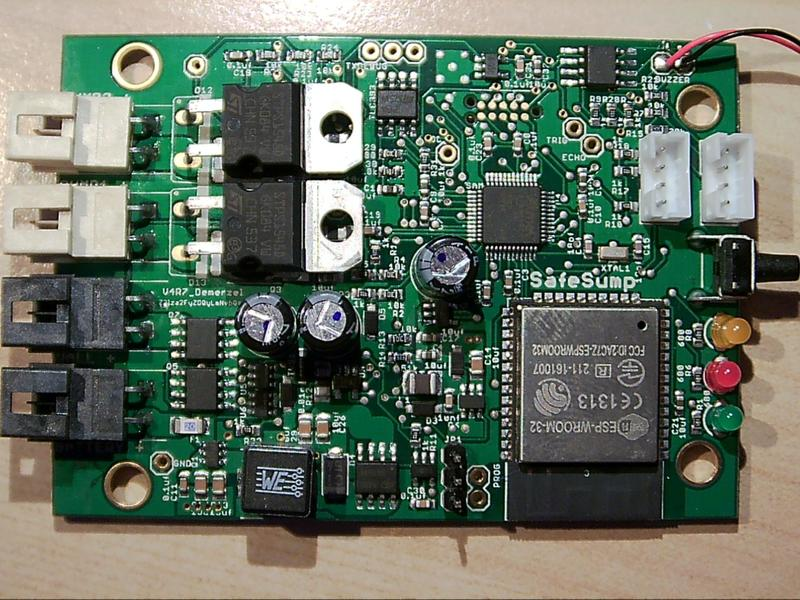
\includegraphics[height=0.1\textwidth]{image1}
%	}
%	\subfloat[]{
%		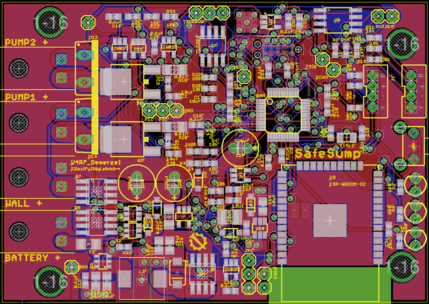
\includegraphics[height=0.1\textwidth]{safesump.png}
%	}
%	\caption*{Controller designed for SafeSump Inc.}
%	\hfill
%\end{figure}

%
%%\begin{figure}[H]
%%	%	\makebox[\textwidth][c]{
%%	\centering
%%	\subfloat[]{
%%		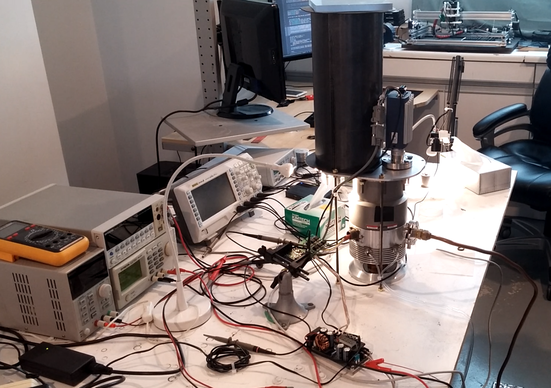
\includegraphics[width=0.5\textwidth]{vacuum}
%%	}\\
%%	\subfloat[]{
%%		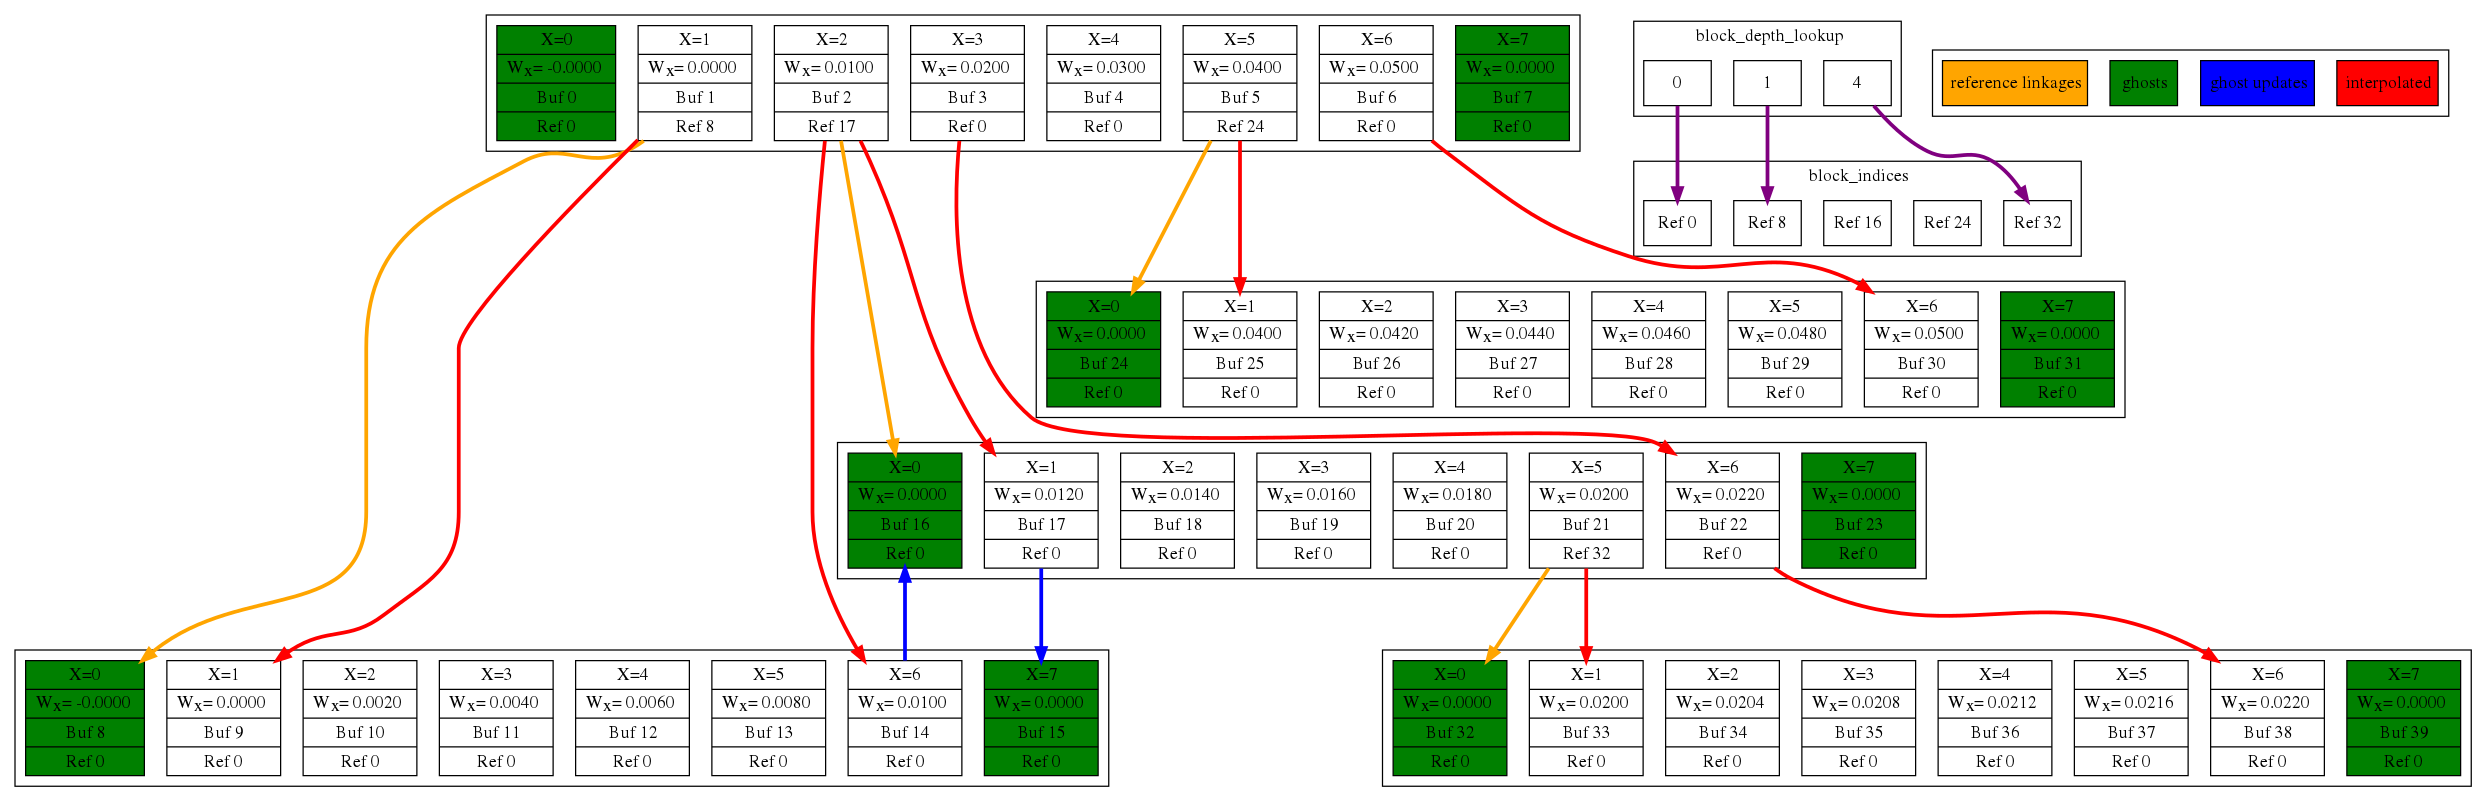
\includegraphics[width=\textwidth]{digraph.png}
%%	}
%%	\caption*{A bespoke high-vacuum system. Data structure diagram for Nyion GPU-accelerated multigrid electrostatics solver for particle-in-cell ion beam simulation.}
%%	\hfill
%%	
%%\end{figure}
%%
%%
%%%
%%%\begin{figure}[H]
%%%	\centering
%%%	
%%%	\subfloat[]{
%%%		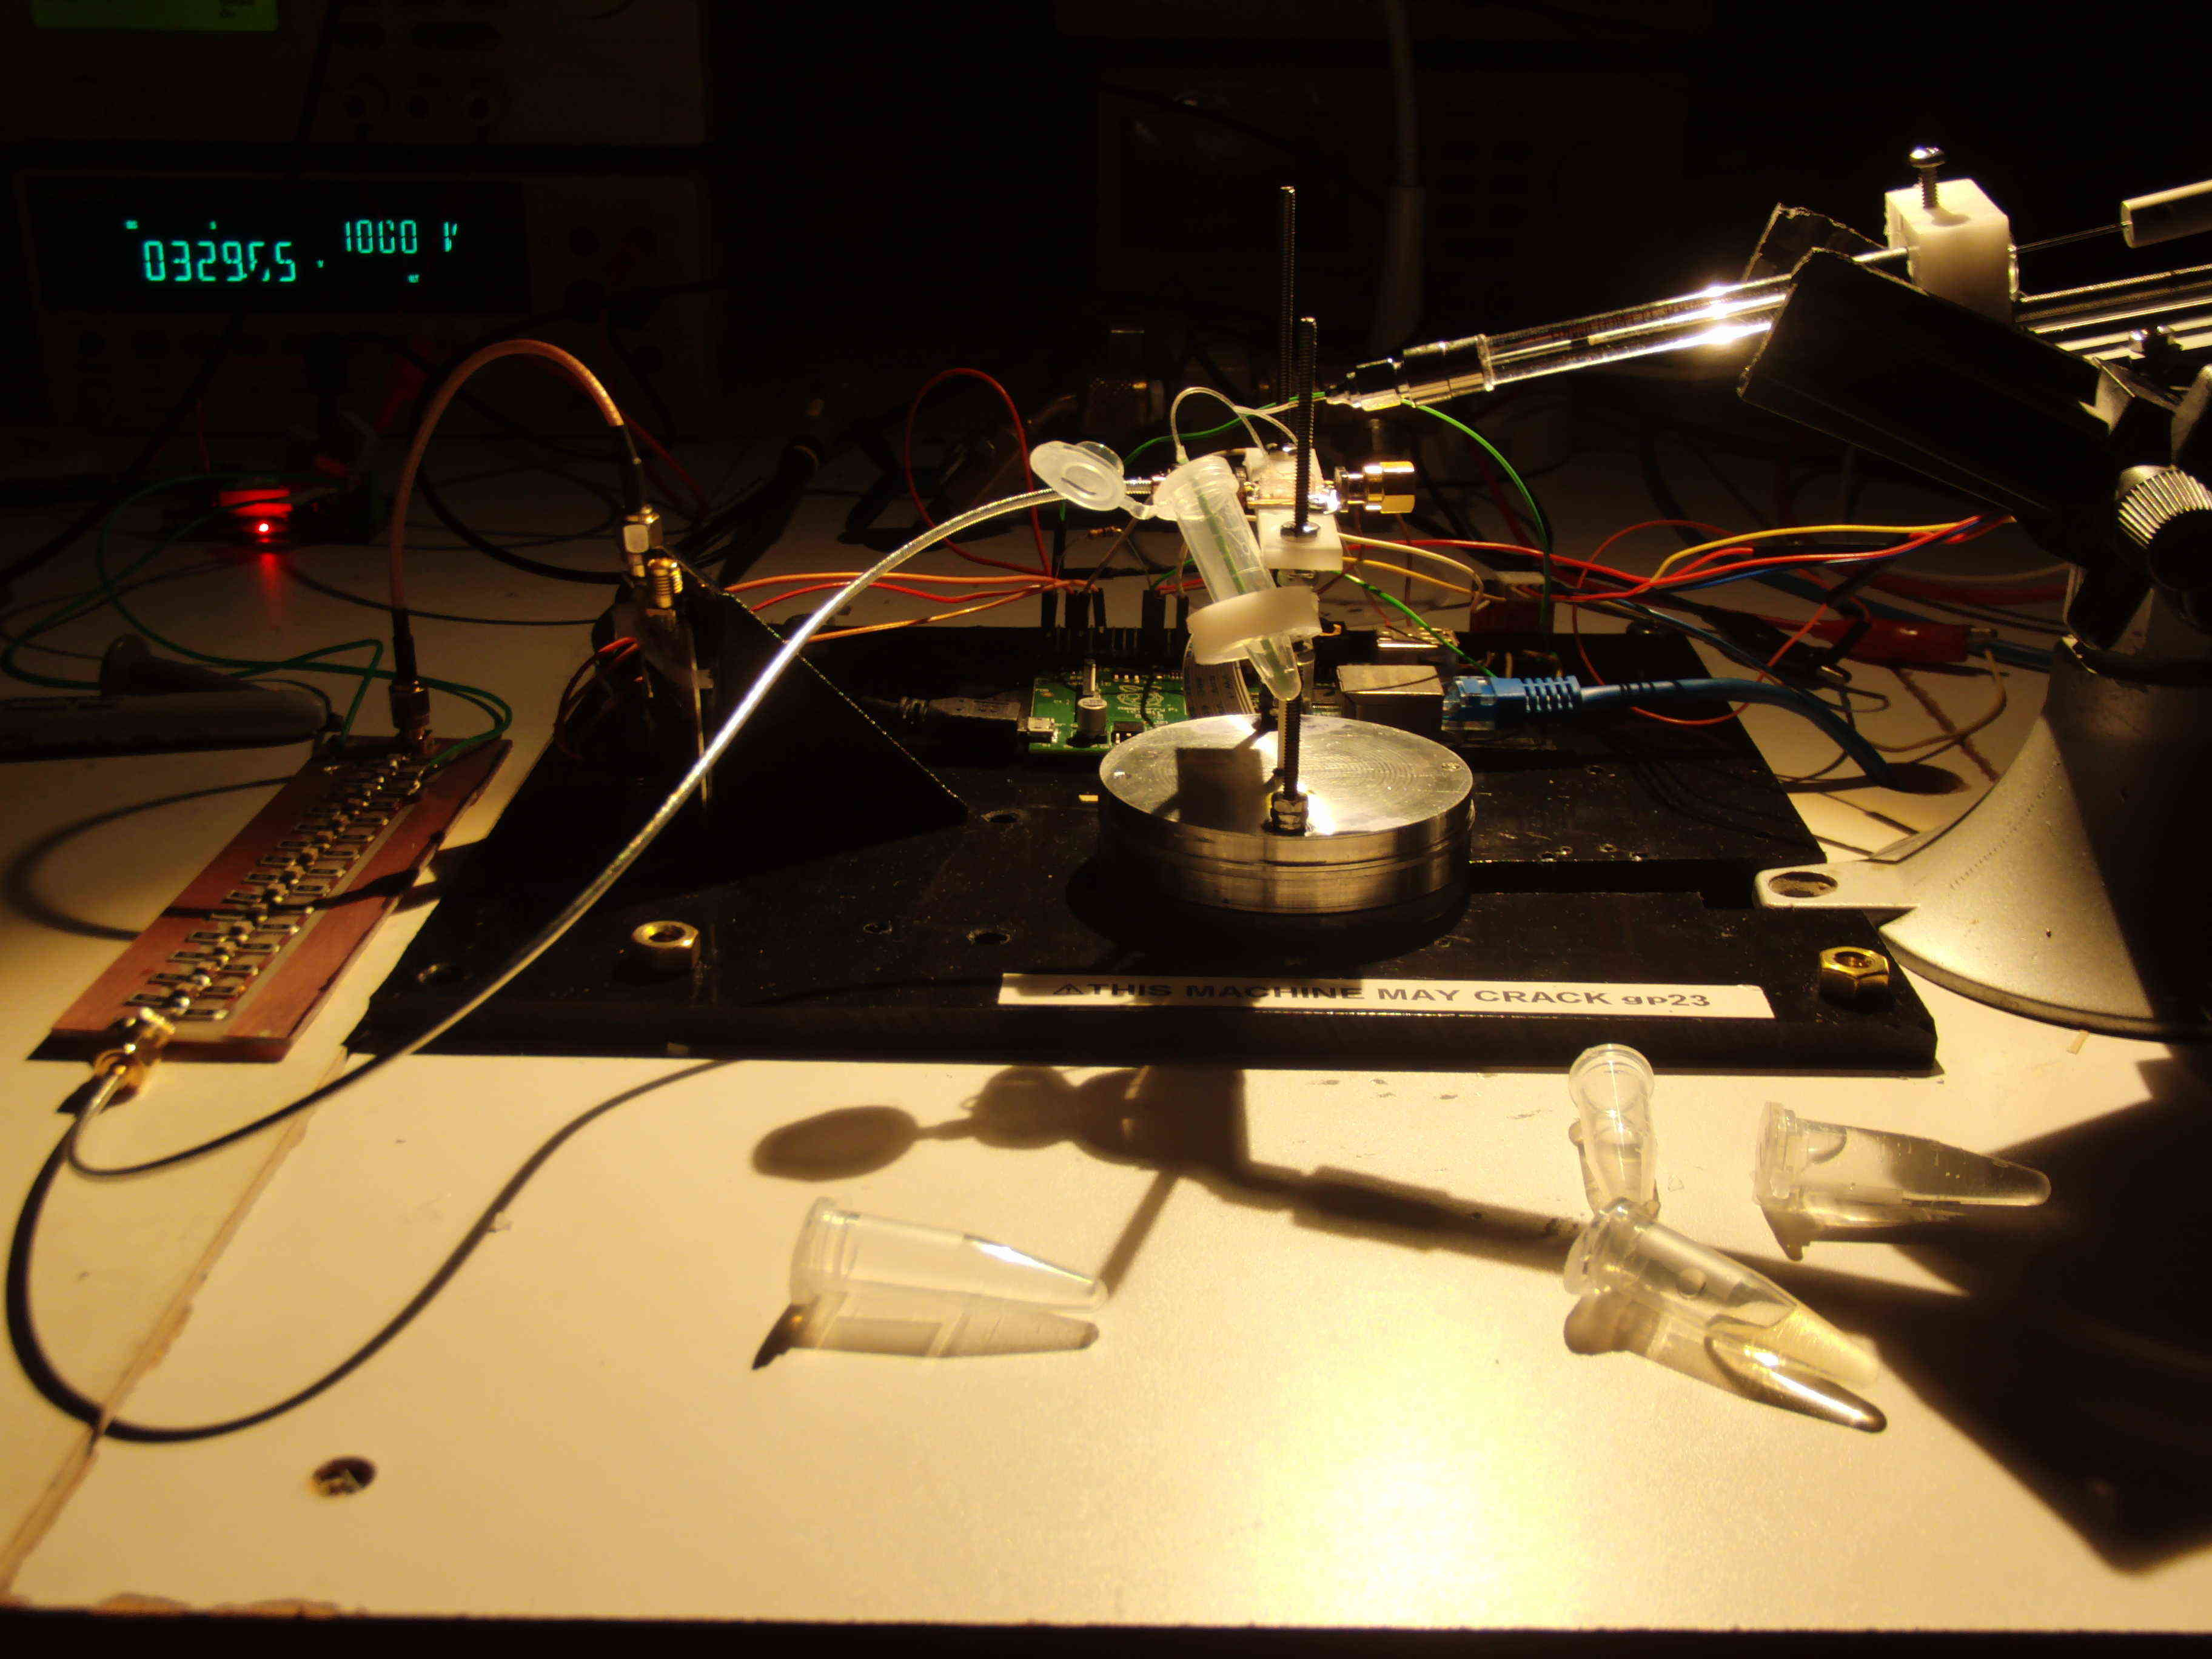
\includegraphics[width=0.5\textwidth]{pulse_exposure_setup}
%%%		
%%%	}
%%%	\subfloat[]{
%%%		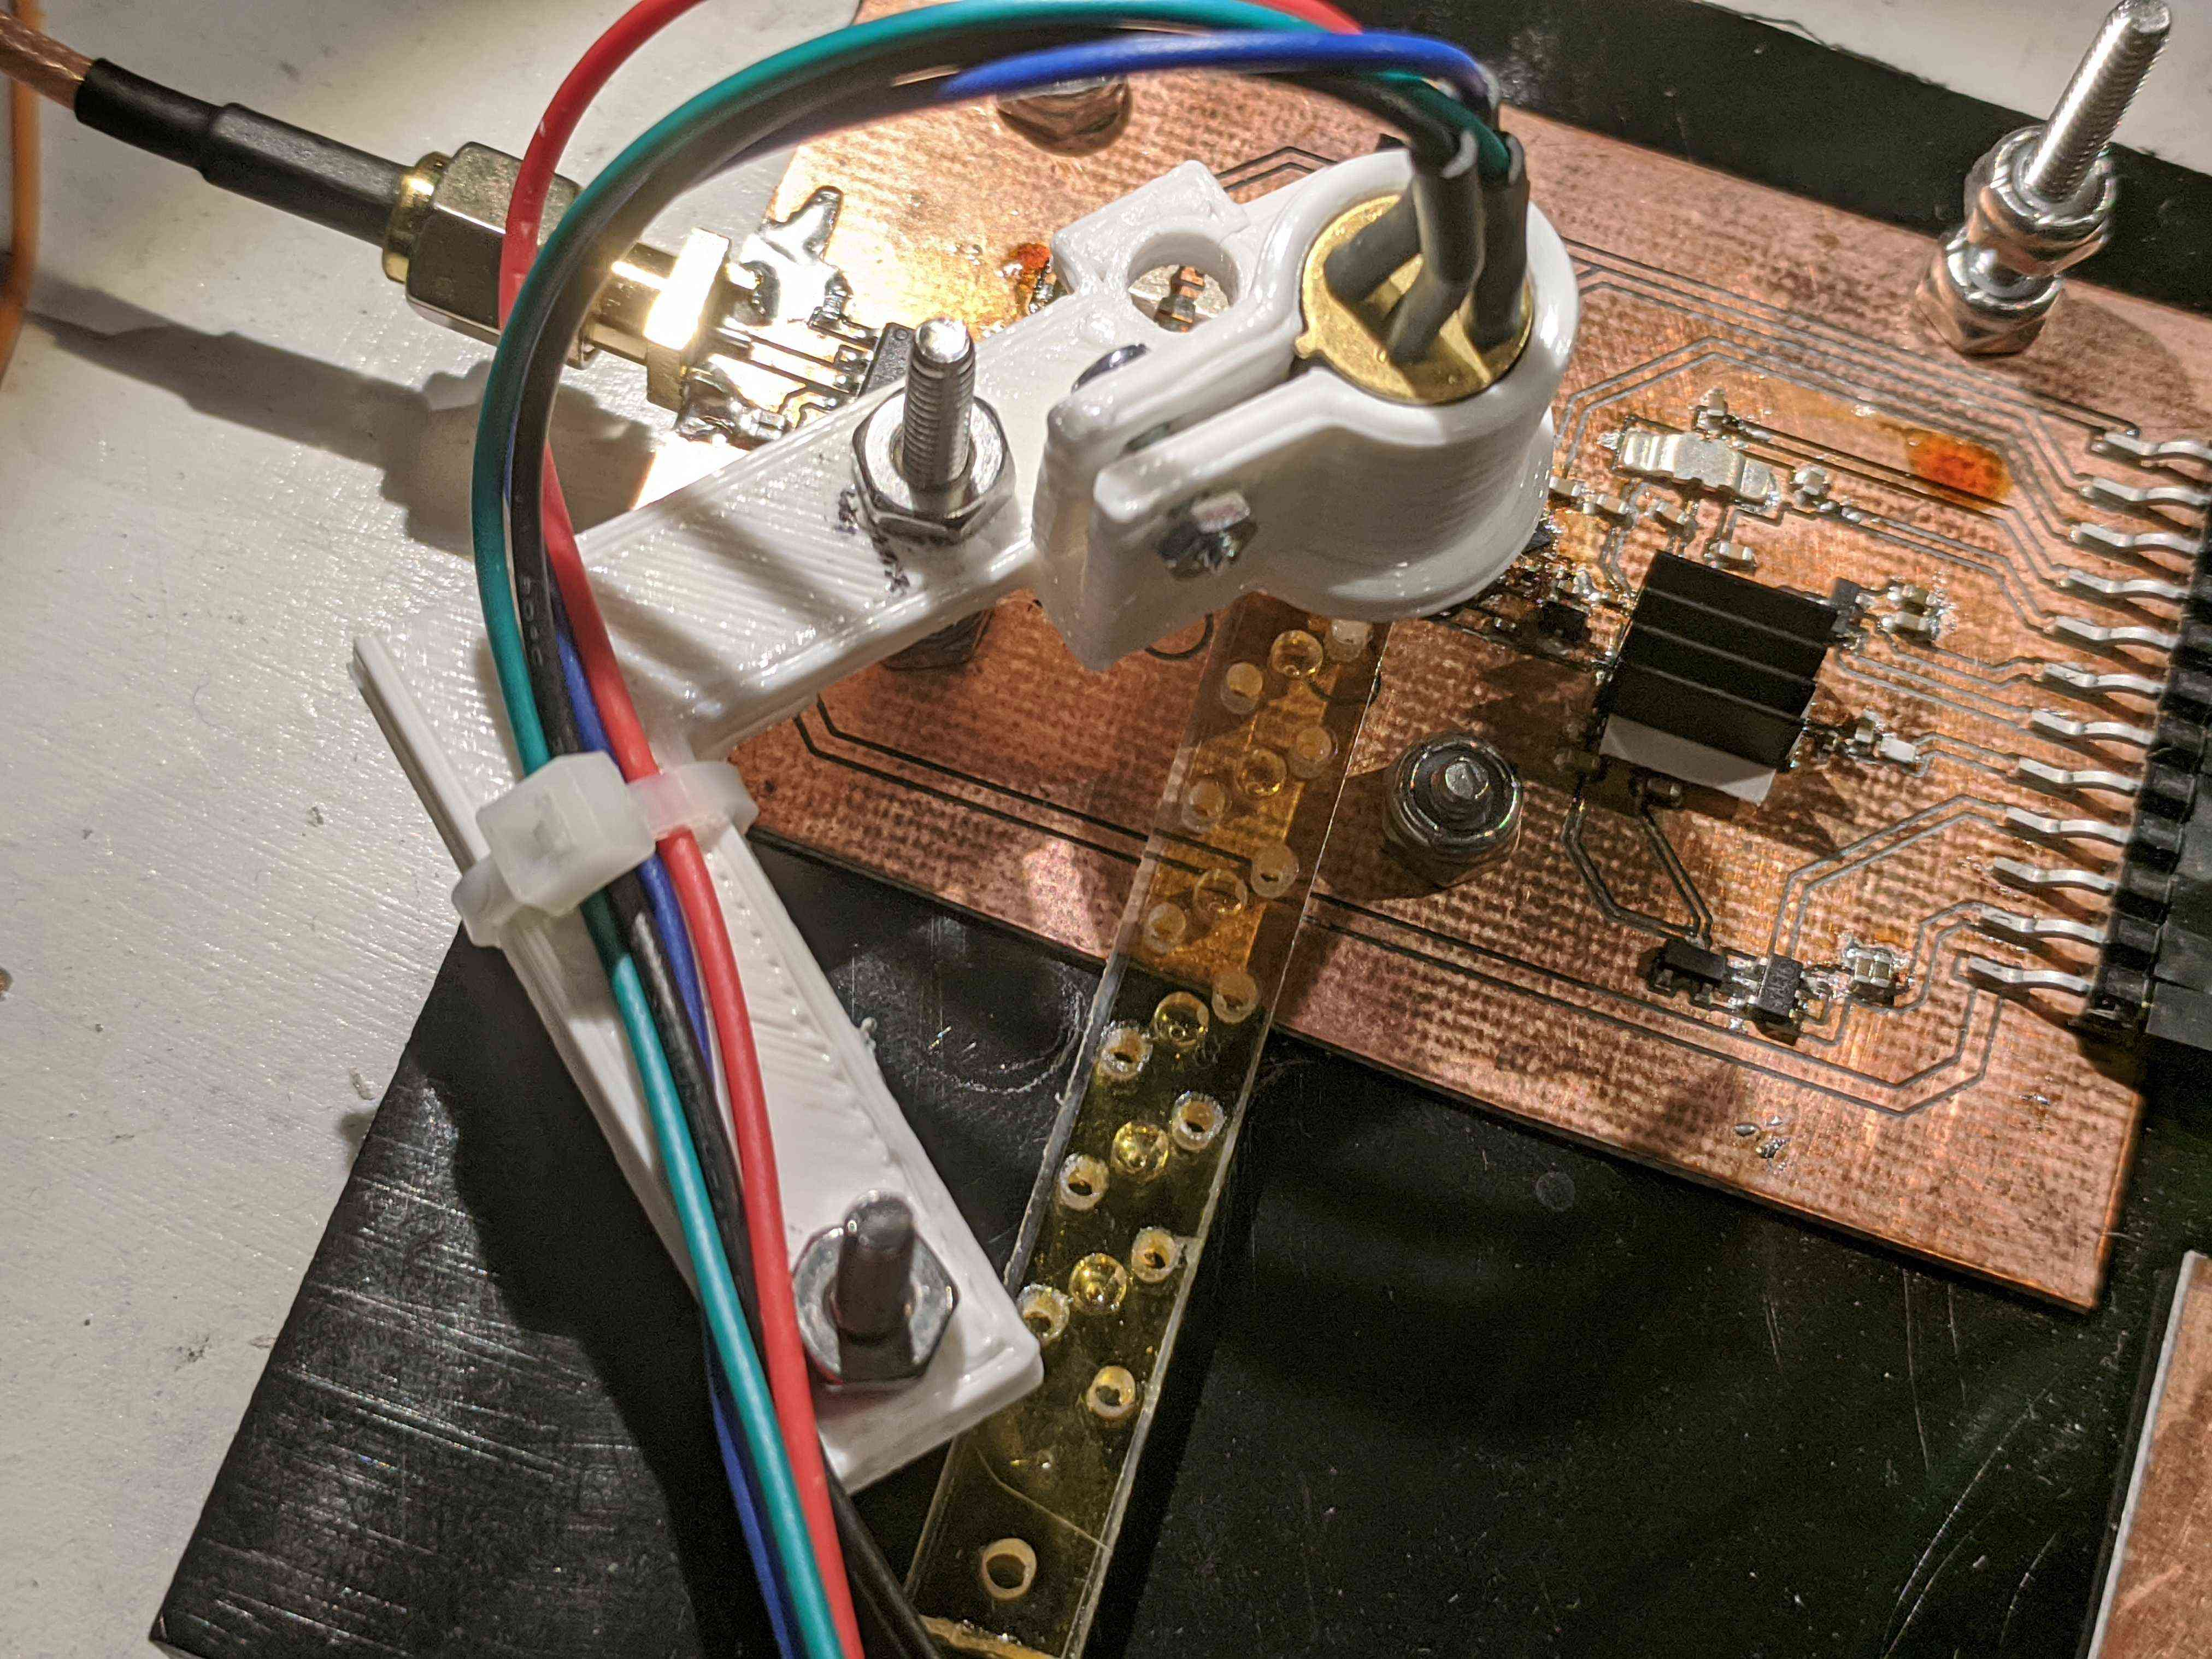
\includegraphics[width=0.5\textwidth]{eppenwolf_2}
%%%	}
%%%	
%%%	\subfloat[]{
%%%		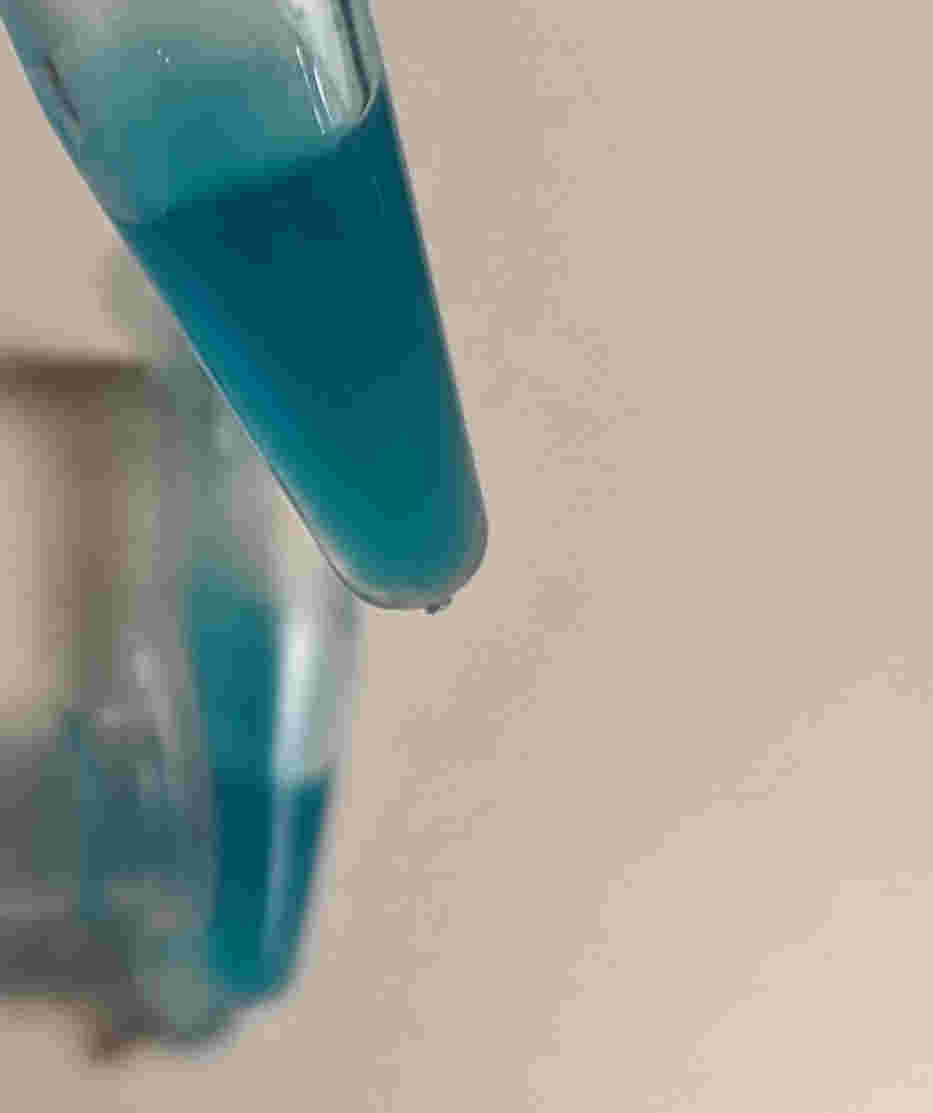
\includegraphics[width=0.4\textwidth]{x_gal.jpg}
%%%	}
%%%	\hfill
%%%	\subfloat[]{
%%%		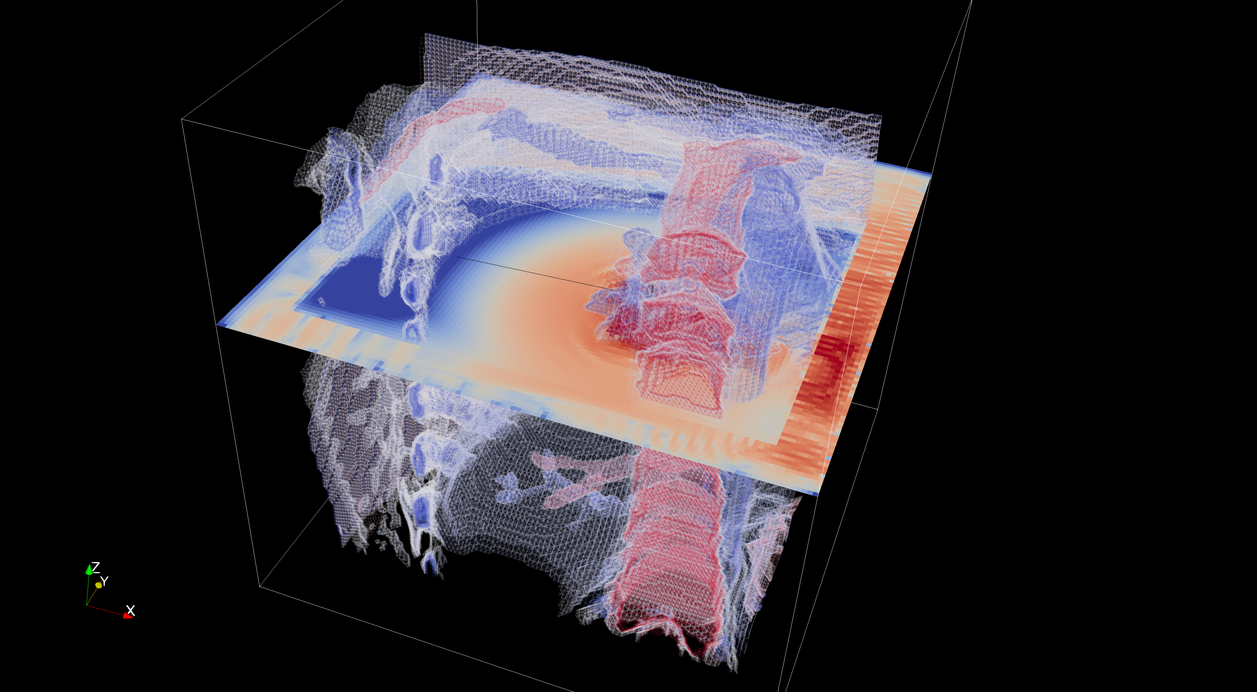
\includegraphics[width=0.5\textwidth]{bronch_9GHz_500W_2}
%%%	}
%%%	
%%%	\caption*{\\ (a) A sub-nanosecond avalanche transistor impulse system. \\ (b) Custom 12 GHz microwave absorption spectrometer described above. \\(c) The very pretty opalescent blue culture caused by E. coli B trying to metabolize lactose in an indicator for the enzyme $\beta$-galactosidase.\\ (d) An FDTD simulation of electromagnetic interaction with tissue. }
%%%\end{figure}
%%%



\end{document}